%
% kurven.tex -- Krümmung eines eindimensionalen Raumes, Einbettung
%
% (c) 2017 Prof Dr Andreas Müller, Hochschule Rapperswil
%
\chapter{Kurven%
\label{skript:chapter:kurven}}
\lhead{Kurven}
\rhead{}
Das Konzept der Krümmung einer Kurve wird bereits im ersten Semester
in der Analysis eingeführt,
die Formeln dafür sollen in diesem Kapitel kurz in Erinnerung gerufen werden.
Wichtiger aber ist die Erkenntnis, dass eine Kurve nur eine sehr simple
innere Geometrie hat.
Nach Wahl eines Anfangspunktes definiert die Bogenlänge entlang der Kurve 
ein Koordinatensystem für die Kurve vollständig.
Die Krümmung der Kurve ist also eine Eigenschaft der Einbettung einer Kurve.

Diese innere Einfachheit von Kurven macht sie zum idealen Werkzeug, mit
dem wir höher\-dimensionale Räume untersuchen können.
Wir können zum Beispiel Dreiecke in einer Fläche untersuchen,
und werden dabei erkennen, dass die Winkelsumme Auskunft geben kann
über die Krümmung der Fläche.
In diesem Kapitel werden wir die Krümmung von Kurven in einer Fläche
studieren, um die Krümmung der Fläche selbst zu charakterisieren.
Dabei werden wir verschiedene Arten von Krümmungsbegriffen finden.
Die mittlere Krümmung hängt von der Einbettung einer Fläche ab und
dient zum Beispiel zur Beschreibung von Minimalflächen in
Kapitel~\ref{chapter:minimal}.
Die Gausskrümmung dagegen ist eine innere Eigenschaft der Fläche und
wird in Kapitel~\ref{skript:chapter:kruemmung} für beliebige Räume
verallgemeinert.

\section{Länge einer Kurve}
\rhead{Definitionen}
Wir betrachten eine Kurve in der Ebene gegeben durch einen Parameterdarstellung
\[
c\colon [a,b] \to\mathbb R^2:t\mapsto c(t).
\]
Darin ist $c(t)$ als Vektor in der Ebene zu betrachten, selbst wenn
wir dies nicht explizit durch Vektorpfeile anzeigen.
\index{Parameterdarstellung!einer Kurve}%
\index{Parametrisierung!einer Kurve}%

Alle unsere Untersuchungen werden die Analysis als Werkzeug verwenden,
wir wollen daher nur Kurven verwenden, für die eine ausreichend glatte
Parametrisierung vorliegt.
Wir verlangen daher, dass die Parameterisierung nach genügend oft nach
dem Parameter abgeleitet werden kann.
Die Ableitung 
\[
v(t)
=
\frac{dc(t)}{dt}
=
\dot c(t)
\]
ist ein Vektor, der im Punkt $c(t)$ tangential ist an die Kurve 
(Abbildung~\ref{skript:kurve:tangente}).
\begin{figure}
\centering
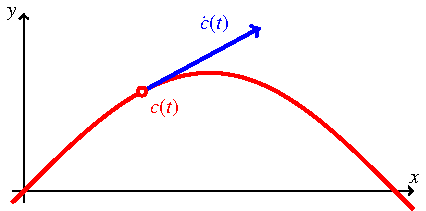
\includegraphics{chapters/tikz/tangente.pdf}
\caption{Kurve $c(t)$ parametrisiert mit dem Parameter $t$ und Tangentialvektor
$\dot c(t)$
\label{skript:kurve:tangente}}
\end{figure}
\index{Tangentialvektor}%

Man kann die Parametrisierung als die Wahl eines Koordinatensystems
für die Kurve interpretieren.
Es stellt sich daher die Frage, inwieweit Aussagen über die Kurve von
der Wahl dieses Koordinatensystems abhängig sind.

In $\mathbb R^2$ haben wir eine Längenmessung zur Verfügung, welche
wir dazu verwenden können, die Länge der Kurve zu berechnen.
Dazu betrachten wir zwei benachbarte Punkte $c(t)$ und $c(t+\Delta t)$
der Kurve.
Ihre Entfernung ist $|c(t+\Delta t) - c(t)|$.
Um daraus die Länge der Kurve zu berechnen, müssen wir die Kurve
an den Stellen $t_1,t_2,\dots,t_n$
beliebig fein in Teile aufteilen und die Längen der Teilstrecken
aufaddieren.
Die Summe
\[
l\simeq\sum_{k=1}^{n-1} |c(t_{i+1})-c(t_i)|
\]
ist daher eine Approximation für die Länge der Kurve.
Die Differenzen können wir mit Hilfe der Ableitung durch
\[
c(t_{i+1})-c(t_i) = \dot c(t_i)\cdot (t_{i+1}-t_i)
\]
approximieren.
Beim Grenzübergang zu einer beliebig feinen Unterteilung wird daraus
das Integral
\begin{equation}
l=\int_a^b |\dot c(t)|\,dt.
\end{equation}
Die Funktion
\begin{equation}
s(t)
=
\int_a^t |\dot c(\tau)|\,d\tau
\label{skript:kurve:s(t)}
\end{equation}
berechnet die Länge der Kurve zwischen den Parameterwerten
$a$ und $t$, insbesondere ist $s(0)=0$.
Die Funktion $s(t)$ ist die {\em Bogenlänge} entlang der Kurve.
\index{Bogenlänge}%

\section{Bogenlängenparameter}
\rhead{Bogenlängenparameter}
\index{Bogenlängenparameter}%
In diesem Abschnitt soll illustriert werden, dass wir bei der Wahl
einer Parametrisierung ein und derselben Kurve zwar viel Freiheit haben,
dass jedoch für geometrische Untersuchungen sich meistens gewisse
Parametrisierungen besonders eignen.
Sowohl hier als auch später beim Studium der Geodäten ist eine
Parametrisierung mit der Bogenlänge besonders nützlich.

\subsubsection{Ein Beispiel}
Wir betrachten die folgenden beiden Parametrisierungen einer ebenen Kurve:
\begin{equation}
\begin{aligned}
c_1\colon
[-1,1]\to\mathbb{R}^2
&\colon
t\mapsto\begin{pmatrix}t\\\sqrt{1-t^2}\end{pmatrix}
&&\text{und}&
c_2\colon
[0,\pi]\to\mathbb{R}^2
&
\colon
s\mapsto\begin{pmatrix}-\cos s\\\sin s\end{pmatrix}.
\end{aligned}
\end{equation}
Beide beschreiben den Einheitskreisbogen, der den Punkt $(-1,0)$ mit
dem Punkt $(1,0)$ verbindet (Abbildung \ref{skript:1dim:kreisbogen}).
\index{Einheitskreis}%
Die Parametrisierungen unterscheiden sich aber in der Ableitung,
die Tangentialvektoren für die beiden Ableitungen sind
\begin{equation}
\begin{aligned}
\frac{dc_1}{dt}
&=
\begin{pmatrix}
1\\-\frac{t}{\sqrt{1-t^2}}
\end{pmatrix}
&&\text{und}&
\frac{dc_2}{ds}
&=
\begin{pmatrix}
\sin s\\\cos s
\end{pmatrix}.
\end{aligned}
\end{equation}
Der Tangentialvektor hat in der zweiten Parametrisierung konstant
die Länge $1$, während sie in der ersten Parametrisierung nahe bei
$t=\pm1$ über alle Grenzen wächst.
\begin{figure}
\centering
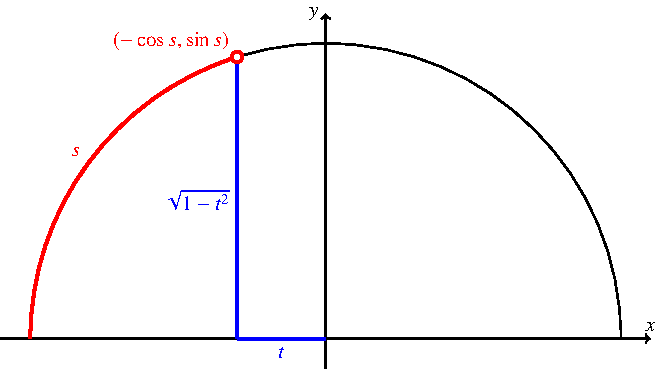
\includegraphics{chapters/tikz/kreisbogen.pdf}
\caption{Kreisbogen zwischen $(-1,0)$ und $(1,0)$. Im Text werden
zwei verschiedene Parametrisierungen dafür vorgestellt.
\label{skript:1dim:kreisbogen}}
\end{figure}

Wir verwenden \eqref{skript:kurve:s(t)}, um die Bogenlänge für die
Parametrisierung $c_1$ zu berechnen.
Dazu berechnen wir
\[
s(t)
=
\int_{-1}^t \sqrt{1+\frac{t^2}{1-\tau^2}}\,d\tau
=
\int_{-1}^t \sqrt{\frac{1-t^2  +t^2}{1-\tau^2}}\,d\tau
=
\int_{-1}^t \frac{1}{\sqrt{1-t^2}} \,d\tau
=
\arcsin t + \frac{\pi}2.
\]

\subsubsection{Bogenlänge als Lösung einer Differentialgleichung}
\index{Bogenlänge!als Lösung einer Differentialgleichung}%
Interpretieren wir den Parameter $t$ als die Zeit der Bewegung eines 
Teilchens entlang der Kurve, dann ist die zeitliche Änderung der Strecke,
die das Teilchen zurück gelegt hat, gerade die Länge des
Geschwindigkeitsvektors, also
\index{Geschwindigkeit}%
\[
\frac{d}{dt} s(t) = \biggl|\frac{d}{dt}c(t)\biggr| = |\dot c(t)|.
\]
Die Funktion $s(t)$ ist also die Lösung der Differentialgleichung
\begin{equation}
\dot s(t)=|\dot c(t)|
\quad
\text{ mit der Anfangsbedingung }\quad s(a)=0.
\label{skript:kruemmung:laengedgl}
\end{equation}
Da $|\dot c(t)|$ eine stetige Funktion ist, können wir nach allgemeinen
Sätzen der Theorie der gewöhnlichen Differentialgleichungen davon ausgehen,
dass diese Differentialgleichung eine eindeutig bestimmte Lösung hat.

Die Lösung der Differentialgleichung \eqref{skript:kruemmung:laengedgl} kann 
durch Integrieren sofort gefunden werden, sie ist
\begin{equation}
s(t)
=
\int_a^t \dot s(\tau)\,d\tau
=
\int_a^t |\dot c(\tau)| \,d\tau
=
\int_a^t \sqrt{\dot x(\tau)^2 + \dot y(\tau)^2}\,d\tau,
\label{skript:kruemmung:laenge}
\end{equation}
wie man auch durch Ableiten nach $t$ sofort nachprüfen kann.
Dies stimmt natürlich mit der Bogenlängenformel~\eqref{skript:kurve:s(t)}
überein.

\subsubsection{Charakterisierung von Bogenlängenparametrisierung}
Verlangen wir von der Kurvenparametrisierung $c(t)$ zusätzlich,
dass $|\dot c(t)|\ne 0$ für alle Parameterwerte $t$, dann ist
die Funktion
$s(t)$
wie in \eqref{skript:kruemmung:laenge} definiert
sogar eine streng monoton wachsende Funktion, insbesondere
kann sie invertiert werden.
Wir können daher zu jedem gegebenen Wert der Länge $s$ durch
Anwendung der inversen Funktion sofort einen Parameterwert $t$
finden, bei dem der Wert $s$ der Länge erreicht wird, also
$s(t)=s$.
Wir schreiben diesen Wert auch abgekürzt als $t(s)$, dies ist eine
übliche, vereinfachte Notation für die inverse Funktion von $s(t)$.
Die Ableitung der Funktion $t(s)$ ist
\begin{equation}
\frac{d}{ds} t(s) = \frac{1}{\dot s(t(s))} = \frac1{|\dot c(t(s))|}
\label{skript:kruemmung:abllaengeinv}
\end{equation}
nach der Formel für die Ableitung der inversen Funktion.

Zu einer beliebigen differenzierbaren Kurve mit der Eigenschaft
$|\dot c(t)|\ne 0$ können wir also immer eine neue Parametrisierung
$c(s)=c(t(s))$ finden, welche die Eigenschaft hat, dass $s$ die
Länge entlang der Kurve gerade die Bogenlänge ist, die durchlaufen
wird.
Wir nennen $s$ auch den {\em Bogenlängenparameter} entlang der Kurve.
\index{Bogenlängenparameter}%
Wir sagen auch, $c(s)$ ist durch die Bogenlänge parametrisiert.
\index{Bogenlänge}%

Die neue Parametrisierung hat als ``Geschwindigkeitsvektor''
\index{Geschwindigkeit}%
\[
\frac{d}{ds} c(s)
=
\frac{d}{ds} c(t(s))
=
\dot c(t(s)) \frac{d}{ds}t(s),
\]
seine Länge wird unter Verwendung von
\eqref{skript:kruemmung:abllaengeinv}
\[
\biggl|
\frac{d}{ds} c(s)
\biggr|
=
\biggl|\dot c(t(s))\frac1{|\dot c(t(s))|}\biggr|
=
1.
\]
Bei Verwendung eines Bogenlängenparameters wird der Tangentialvektor
immer ein Einheitsvektor sein.

Umgekehrt wird die Differentialgleichung \eqref{skript:kruemmung:laengedgl}
besonderes einfach, wenn $|\dot c(t)|=1$ ist, nämlich $\dot s(t)=1$ mit
der Lösung $s(t)=t$.
Die Bedingung $|\dot c(t)|=1$ charaktersiert also $t$ als einen
Bogenlängenparameter.

\subsubsection{Beispiele}
\begin{beispiel}
Wir betrachten eine Gerade 
\[
c(t)=\vec p + t\vec v,\qquad \vec v\ne 0
\]
in der Ebene.
Wir legen $a=0$ willkürlich fest.
Die Differentialgleichung~\eqref{skript:kruemmung:laengedgl} für die
Kurven\-längen\-funktion $s(t)$ wird
\[
\dot s(t) = |\dot c(t)| = |v|
\]
mit der Lösung
\[
s(t)=|v|t.
\]
Da $v\ne 0$ ist $s(t)$ monoton wachsend und wir können sofort nach
$t$ auflösen, es ist
\[
t(s)=\frac{s}{|\vec v|}.
\]
Setzen wir dies in die ursprüngliche Parametrisierung ein, erhalten
wir
\[
c(s)
=
c(s(t))
=
\vec p + t(s)\vec v
=
\vec p + \frac{s}{|\vec v|}\vec v
=
\vec p + s\frac{v}{|v|},
\]
Die Ableitung nach $s$ hiervon ist ein Einheitsvektor, wie zu erwarten
war.
\end{beispiel}

\begin{beispiel}
Wir parametrisieren den Einheitskreis mit Hilfe der $x$-Koordinate, also
durch
\[
c\colon
[-1,1]\to\mathbb R^2
\colon
t\mapsto (-t,\sqrt{1-t^2}).
\]
Ganz offensichtlich ist dies kein Bogenlängenparameter.
Für die Bogenlänge brauchen wir die Ableitung nach dem Parameter $t$,
sie ist
\[
\dot c(t)=\biggl(-1, -\frac{t}{\sqrt{1-t^2}}\biggr).
\]
Die Bogenlänge ist das Integral der Länge der Ableitung:
\[
s(t)
=
\int_{-1}^t \sqrt{1 + \frac{\tau^2}{1-\tau^2}}\,d\tau
=
\int_{-1}^t \sqrt{\frac{1-\tau^2 +\tau^2}{1-\tau^2}}\,d\tau
=
\int_{-1}^t \frac{1}{\sqrt{1-\tau^2}}\,d\tau
\]
Das Integral auf der rechten Seite kann man in geschlossener
Form auswerten, es ist
\[
s(t)=\arcsin(t) + \frac{\pi}{2}
\]
mit der inversen Funktion
\[
t(s)
=
\sin\biggl(s-\frac{\pi}2\biggr)
=
-\cos(s).
\]
Setzen wir dies in die Parametrisierung ein, erhalten wir
\[
c(s)
=
\bigl(\cos(s), \sqrt{1-\cos^2(s)}\bigr)
=
(\cos(s), \sin(s)),
\]
also die übliche Parametrisierung des Einheitskreises mit Hilfe
des Winkels.
Der Winkel muss in Bogenmass gemessen werden, also der Länge entlang
des Kreises.
\end{beispiel}

Da sich jede beliebige Kurve mit einem Bogenlängenparameter versehen
lässt, können wir für je zwei beliebige Kurven immer eine Abbildung
zwischen den Kurven definieren, die Punkte mit gleichem Bogenlängenparameter
zur Deckung bringt.
Zwei Kurven sind also nicht mehr unterscheidbar, wenn sie mal mit
einem Bogenlängenparameter ausgestattet sind.
Verbleibende Unterschiede zwischen Kurven entstehen einzig durch die
Einbettung der Kurve im Raum.

Für eine Ameise, die ausschliesslich auf der Kurve lebt, ist die Länge,
die sie entlang der Kurve zurückgelegt hat, die einzige geometrische
Information, die ihr zugänglich ist.
Sie kann verschiedene Kurven im Raum nicht voneinander unterscheiden.

\section{Krümmung%
\label{section:kurve:kruemmung}}
%\rhead{Krümmung}
\begin{figure}
\centering
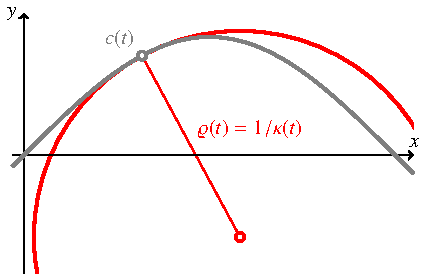
\includegraphics{chapters/tikz/kruemmung.pdf}
\caption{Krümmung $\kappa(t)$ und Krümmungsradius $\varrho(t)$
der Sinus-Kurve im Punkt $c(t)$
\label{skript:kurven:fig:kruemmung}}
\end{figure}
Wir möchten in diesem Abschnitt zeigen, dass die Krümmung einer Kurve
ausschliesslich eine Eigenschaft der Einbettung der Kurve in den
Raum ist.
Wir tun das, indem wir davon ausgehen, dass eine Kurve bereits mit
der Bogenlänge parametrisiert ist, dass wir also die Standardparametrisierung
gewählt haben, in der über die innere Geometrie der Kurve verfügbare
Information bereits vollständig verwertet worden ist.

\rhead{Krümmung}

Eine Gerade zeichnet sich dadurch aus, dass der Tangentialvektor in
der Bo\-gen\-län\-gen\-pa\-ra\-me\-tri\-sie\-rung nicht ändert.
Eine Gerade ist nicht gekrümmt.
Krümmung ist also die Änderung des Tangentialvektors oder
\[
\kappa(s)=|\ddot c(s)|.
\]
\index{Krümmung!einer Kurve}%
Das nachfolgende Beispiel und die Abbildung~\ref{skript:kurven:fig:kruemmung}
zeigen, dass eine Kurve mit Krümmung $\kappa(s)$ durch einen Kreis mit
Radius $1/\kappa(s)$, den sogenannten Krümmungskreis, approximiert wird.
\index{Krümmungskreis}%

\begin{beispiel}
Der Kreis mit Radius $r$ kann parametrisiert werden durch die Funktion
\[
s\mapsto c(s)=\biggl( r\cos\frac{s}{r}, r\sin\frac{s}{r}\biggr).
\]
Die Ableitung ist
\[
\dot c(s)=\biggl(-\sin\frac{s}{r},\cos\frac{s}{r}\biggr)
\qquad\Rightarrow\qquad
|\dot c(s)|
=
\sqrt{\cos^2\frac{s}{r}+\sin^2\frac{s}{r}}=1,
\]
dies ist also eine Parametrisierung mit Bogenlängenparameter.
Die Krümmung ist der Betrag der zweiten Ableitung, also
\[
\ddot c(s)=\biggl(-\frac1r\cos\frac{s}{r},-\frac1r\sin\frac{s}{r}\biggr)
\qquad\Rightarrow\qquad
\kappa(s)
=
|\ddot c(s)|
=
\frac1r.
\]
Der Kreis mit Radius $r$ ist also eine Kurve mit konstanter Krümmung
$\kappa(s)=\frac1r$.
\end{beispiel}

Ist die Kurve nicht durch die Bogenlänge parametrisiert, wird die
Berechnung der Krümmung etwas komplizierter.
Es muss aber immer noch gelten, dass $\kappa(t)$ die Änderung des
Einheitstagentialvektors pro Längeneinheit entlang der Kurve angibt.
Es ist also zu berechnen
\begin{equation}
\kappa(t)
=
\underbrace{\frac{1}{|\dot c(t)|}}_{\text{pro Längeneinheit}}
\cdot\;
\biggl|\frac{d}{dt}\underbrace{\frac{\dot c(t)}{|\dot c(t)|}}_{\text{Einheitstangentialvektor}}\biggr|.
\label{skript:kruemmung:krallg2}
\end{equation}
Die Berechnung ist etwas mühsam wegen des Vektorbetrages im Nenner.
Wir berechnen daher zuerst die Ableitung von $|\dot c(t)|$ mit
Hilfe der Kettenregel:
\begin{align*}
\frac{d}{dt}|\dot c(t)|
&=
\frac{d}{dt}\sqrt{\dot x(t)^2+\dot y(t)^2}
=
\frac1{2\sqrt{\dot x(t)^2 + \dot y(t)^2}}(2\dot x(t)\ddot x(t) + 2\dot y(t)\ddot y(t))
\\
&=
\frac{1}{|\dot c(t)|}
\begin{pmatrix}\dot x(t)\\\dot y(t)\end{pmatrix}
\cdot
\begin{pmatrix}\ddot x(t)\\\ddot y(t)\end{pmatrix}
=
\frac{1}{|\dot c(t)|}
\dot c(t)\cdot\ddot c(t)
=
\frac{\dot c(t)}{|\dot c(t)|} \cdot\ddot c(t).
\end{align*}
Damit können wir jetzt auch die Ableitung des Einheitstangentialvektors
berechnen:
\begin{align}
\frac{d}{dt} \frac{\dot c(t)}{|\dot c(t)|}
&=
\frac{\displaystyle\ddot c(t) |\dot c(t)| - \dot c(t) \frac{d}{dt}|\dot c(t)|}{|\dot c(t)|^2}
=
\frac{\displaystyle\ddot c(t) |\dot c(t)| - \dot c(t) \frac{\dot c(t)}{|\dot c(t)|}\cdot \ddot c(t)}{|\dot c(t)|^2}
=
\frac{\displaystyle\ddot c(t) - \frac{\dot c(t)}{|\dot c(t)|} \left( \frac{\dot c(t)}{|\dot c(t)|}\cdot \ddot c(t)\right)}{|\dot c(t)|}.
\label{skript:kruemmung:krallg1}
\end{align}
\begin{figure}[t!]
\centering
\subfigure{}{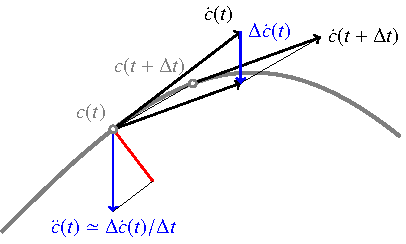
\includegraphics[]{chapters/tikz/kruemmung2.pdf}}
\hfill
\subfigure{}{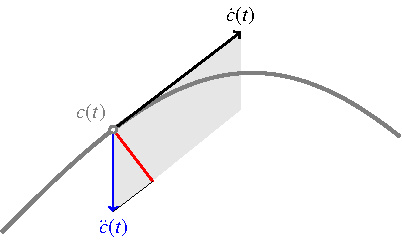
\includegraphics[]{chapters/tikz/kruemmung3.pdf}}
\caption{Berechnung der Krümmung aus den ersten zwei Ableitungen
$\dot c(t)$ und $\ddot c(t)$ der Kurve.
Die Krümmung ist proportional zur Projektion der zweiten Ableitung
$\ddot c(t)$ auf die Normale auf der Tangentenrichtung $\dot c(t)$.
Die Projektion ist in beiden Abbildungen {\color{red}rot} eingezeichnet.
Auf der rechten Abbildung sieht man, dass dies auch die Höhe des
von $\dot c(t)$ und $\ddot c(t)$ aufgespannten Parallelogramms ist.
\label{skript:chapter:kruemmungsberechnung}}
\end{figure}%
Schreiben wir den Einheitstangentialvektor
\[
e(t)= \frac{\dot c(t)}{|\dot c(t)|},
\]
wird der Zähler etwas übersichtlicher zu
\[
\ddot c(t) - \frac{\dot c(t)}{|\dot c(t)|} \biggl( \frac{\dot c(t)}{|\dot c(t)|}\cdot \ddot c(t)\biggr)
=
\ddot c(t) - e(t)\; \bigl(e(t)\cdot \ddot c(t)\bigr).
\]
Da $e(t)$ ein Einheitsvektor ist, ist
$e(t) \;(e(t)\cdot\ddot c(t))$ die Projektion des Vektors
$\ddot c(t)$ auf den Vektor $e(t)$
(Abbildung~\ref{skript:chapter:kruemmungsberechnung} links).
Der Zähler ist also die Komponenten von $\ddot c(t)$ senkrecht auf dem
Tangentialvektor.
Wir brauchen davon aber nur den Betrag, also die Höhe des Parallelograms
mit den Seiten $e(t)$ und $\ddot c(t)$
(Abbildung~\ref{skript:chapter:kruemmungsberechnung} rechts).
Diese können wir aber auch dadurch erhalten, dass wir den orientierten
Parallelogramminhalt berechnen und durch die Länge der Grundseite
$e(t)$ teilen, die aber ein Einheitsvektor ist.
Den Parallelogramminhalt können wir mit der Determinante berechnen:
\[
\biggl|\ddot c(t) - \frac{\dot c(t)}{|\dot c(t)|}
\biggl(\frac{\dot c(t)}{|\dot c(t)|} \cdot \ddot c(t)\biggr)\biggr|
=
\det \biggl(\frac{\dot c(t)}{|\dot c(t)|}, \ddot c(t)\biggr)
=
\frac1{|\dot c(t)|}\det (\dot c(t),\ddot c(t)).
\]
Daraus können wir jetzt auch eine Formel für die Krümmung zusammensetzen.
Zunächst müssen wir den Faktor $|\dot c(t)|$ im Nenner wieder
hinzufügen, den wir in~\eqref{skript:kruemmung:krallg1} gefunden hatten.
Ausserdem brauchen wir einen weiteren Faktor $|\dot c(t)|$ im Nenner
aus der Definition~\eqref{skript:kruemmung:krallg2}.
Damit wird
\begin{equation}
\kappa(t)
=
\frac{\det(\dot c(t),\ddot c(t))}{|\dot c(t)|^3}
\label{skript:kruemmung:krkurveallg}
\end{equation}
die allgemeine Formel für die Krümmung einer ebenen Kurve.


\begin{beispiel}
\index{Ellipse!Krümmung}%
Wir berechnen die Krümmung einer {\em Ellipse mit den Halbachsen
$a$ und $b$} und verwenden dazu die Parametrisierung mit Hilfe des
Zentriwinkels, also
\[
c
\colon
[0,2\pi]\to\mathbb R^2
\colon
t\mapsto c(t) = (a\cos t, b \sin t).
\]
Nach der Formel~\eqref{skript:kruemmung:krkurveallg} brauchen wir zunächst
die ersten beiden Ableitungen, diese sind
\begin{align*}
\dot c(t)
&=
(-a\sin t, b\cos t)
\\
\ddot c(t)
&=
(-a\cos t, -b\sin t)
\end{align*}
Die Determinante von $\dot c(t)$ und $\ddot c(t)$ ist
\[
\det(\dot c(t), \ddot c(t))
=
\left|\begin{matrix}
-a\sin t & -a \cos t\\
 b\cos t & -b \sin t
\end{matrix}\right|
=
ab\sin^2t+ab\cos^2 t
=
ab.
\]
Die Krümmung ist daher
\[
\kappa(t)
=
\frac{ab}{(a^2\sin^2 t + b^2 \cos^2 t)^{\frac32}}
\]
Da die Faktoren $\sin^2t$ und $\cos^2t$ im Nenner sich zu $1$ summieren,
steht in der Klammer im Nenner ein gewichteter Mittelwert von $a^2$
und $b^2$.
Die Extremwerte des Nenners sind daher $a^3$ und $b^3$, sie werden bei
$t=\pm\frac{\pi}2$ bzw.~$t\in\{0,\pi\}$ angenommen.
Nimmt man an, dass $a>b$ ist, dann wird die maximale Krümmung $t=0$ und
und $t=\pi$ erreicht, sie ist $ab/b^3=a/b^2$.
Die minimale Krümmung wird dagegen bei $t=\pm\frac{\pi}2$ angenommen,
sie ist $ab/a^3=b/a^2$.

Ein Kreis ist eine Ellipse, bei der $a$ und $b$ übereinstimmen.
Für einen Kreis sind die beiden Extremwerte der Krümmung
gleich gross, nämlich
\[
\frac{a}{b^2}=\frac{r}{r^2}=\frac1r
\qquad\text{und}\qquad
\frac{b}{a^2}=\frac{r}{r^2}=\frac1r,
\]
wie wir früher bereits gefunden haben.
\end{beispiel}

\begin{beispiel}
\index{Parabel, Krümmung}%
\index{Krümmung!einer Parabel}%
Für spätere Anwendungen berechnen wir noch die Krümmung einer {\em Parabel},
genauer des Graphen der Funktion
\[
y = ax^2 + bx + c.
\]
Als Parameterdarstellung ausgedrückt geht es also um die Kurve
\[
t\mapsto c(t)
=
\begin{pmatrix}
t\\
at^2+bt+c
\end{pmatrix}.
\]
Davon sind zunächst die Ableitungen nach $t$ zu bestimmen, sie sind
\begin{align*}
\dot c(t)
&=
\begin{pmatrix}1\\2at+b\end{pmatrix},
\\
\ddot c(t)
&=
\begin{pmatrix}0\\2a\end{pmatrix}.
\end{align*}
Die Krümmung ist nach Formel~\eqref{skript:kruemmung:krkurveallg}
\begin{align}
\kappa(t)
&=
\frac{\left|\begin{matrix}1&0\\2at+b&2a\end{matrix}\right|}{
(1+(2at+b)^2)^{\frac32}
}
=
\frac{2a}{(1+(2at+b)^2)^{\frac32}}.
\label{skript:kruemmung:parabelkruemmung}
\end{align}
Der Scheitelpunkt befindet sich bei $t=-b/2a$, an dieser Stelle verschwindet
die innere Klammer im Nenner von~\eqref{skript:kruemmung:parabelkruemmung}.
Am Scheitel ist die Krümmung daher viel einfacher
\begin{equation}
\kappa_{\text{Scheitel}}
=
\kappa\biggl(-\frac{b}{2a}\biggr)
=
2a
\qquad
\Rightarrow
\qquad
\varrho_{\text{Scheitel}}
=
\frac1{\kappa_{\text{Scheitel}}}
=
\frac1{2a}.
\label{skript:kruemmung:parabel:scheitel}
\end{equation}
Der Krümmungsradius im Scheitel der Normalparabel $y=x^2$ ist also
$\varrho=\frac12$.
\end{beispiel}

Für eine Kurve in drei Dimension lässt sich das bei der Herleitung
der Formel~\eqref{skript:kruemmung:krkurveallg} für $\kappa(t)$
verwendete Argument fast unverändert übertragen.
Die einzige Änderung ist an der Stelle erforderlich, wo wir die Determinante
zur Berechnung des orientierten Volumens des Parallelograms verwendet
haben.
In drei Dimensionen muss stattdessen der Betrag des Vektorproduktes 
verwendet werden.
Die Krümmung einer Raumkurve in einer beliebigen Parametrisierung ist
daher
\begin{equation}
\kappa(t)
=
\frac{|\dot c(t)\times \ddot c(t)|}{|\dot c(t)|^3}.
\label{skript:kruemmung:krkurveallg3d}
\end{equation}
Dies ist natürlich identisch mit \eqref{skript:kruemmung:krkurveallg},
wenn man sich die Ebene der Kurve in einen dreidimensionalen Raum
eingebettet vorstellt.

\begin{beispiel}
\begin{figure}
\centering
\includegraphics[width=\hsize]{chapters/3d/kurve.jpg}
\caption{Kurven $t\mapsto(t,t^2,0)$ (rot) und $t\mapsto(t,t^2,t^3)$ (gelb).
\label{skript:kruemmung:fig:kurvekr}}
\end{figure}
Wir betrachten die beiden Kurven
\begin{align*}
c_1(t)&=(t,t^2,0)
&
c_2(t)&=(t,t^2,t^3)
\end{align*}
(Abbildgung~\ref{skript:kruemmung:fig:kurvekr}).
$c_1(t)$ ist eine ebene Kurve, nämlich die Projektion der Raumkurve
$c_2(t)$ in die $x$-$y$-Ebene, sie ist in
Abbildung~\ref{skript:kruemmung:fig:kurvekr} rot dargestellt.
Die Kurve $c_2(t)$ ist in Abbildung~\ref{skript:kruemmung:fig:kurvekr} 
dagegen gelb dargestellt.
Wir wollen von beiden Kurven die Krümmung berechnen.
Dazu berechnen wir zunächst die Ableitungen und das Vektorprodukt
\begin{align*}
\dot c_1(t)
&=
(1,2t,0)
&
\dot c_2(t)
&=
(1,2t,3t^2)
\\
\ddot c_1(t)
&=
(0,2,0)
&
\ddot c_2(t)
&=
(0, 2, 6t)
\\
\dot c_1(t)\times \ddot c_1(t)
&=
(0,0,2)
&
\dot c_2(t)\times \ddot c_2(t)
&=
(6t^2,-6t,2)
\end{align*}
Daraus kann man jetzt die Krümmungen berechnen:
\begin{align*}
\kappa_1(t)
&=
\frac{2}{(1+4t^2)^{\frac32}}
\\
\kappa_2(t)
&=
\frac{2}{(1+4t^2 + 9t^4)^{\frac32}}
\sqrt{1+9t^2+9t^4}
\end{align*}
Für den Parameterwert $t=0$ stimmen die beiden Krümmungen überein.
\end{beispiel}

\section{Rekonstruktion einer ebenen Kurve aus der Krümmung}
%\rhead{Rekonstruktion aus der Krümmung}
Die Krümmung bestimmt eine Kurve in der Ebene eindeutig.
Um dies einzusehen, parametrisieren wir eine ebene Kurve mit
$x$, schreiben also $c(x)=(x,y(x))$.
Wir müssen jetzt nachrechnen, dass die Vorgabe der Krümmung $\kappa(x)$
und der Steigung in einem Punkt die Kurve eindeutig festlegt.
Dazu stellen wir eine Differentialgleichung zweiter Ordnung auf,
allgemeine Sätze über Existenz und Eindeutigkeit der Lösung von
gewöhnlichen Differentialgleichungen werden unsere Aussage dann
als Konsequenz haben.

\rhead{Rekonstruktion aus der Krümmung}

In dieser speziellen Wahl der Parametrisierung ist $x(0)=0$ und $\dot x(0)=1$.
Die Ableitung von $y$ nach dem Parameter ist dann $\dot y=y'(x)$.
Somit wird die Formel für die Krümmung
\[
\kappa(x)
=
\frac{\left|\begin{matrix}\dot x&\ddot x\\\dot y&\ddot y\end{matrix}\right|}{(\dot x^2+\dot y^2)^{\frac32}}
=
\frac{\left|\begin{matrix}1&0\\y'&y''\end{matrix}\right|}{(1+y'^2)^{\frac32}}
=
\frac{y''}{(1+y'(x))^{\frac32}}
\]
oder in expliziter Form:
\[
y''(x)=\kappa(x) (1+y'(x)^2)^{\frac32}.
\]
Dies ist eine gewöhnliche Differentialgleichung zweiter Ordnung.
Da die rechte Seite erfüllt die Bedingungen, die in üblichen
Eindeutigkeitssätzen für gewöhnliche Differentialgleichungen
verlangt werden, daher gibt es genau eine Lösung dieser
Differentialgleichung zu vorgegebenem Anfangspunkt und Anfangsrichtung.
Damit ist gezeigt, dass in der Ebenen zwei Kurven mit der gleichen
Krümmung, gleichem Anfangspunkt und gleicher Anfangsrichtung übereinstimmen
müssen.
Anders formuliert: zwei ebene Kurven mit gleicher Krümmung in Abhängigkeit
von einem Bogenlängenparameter sind kongruent.

In drei Dimensionen kann die Krümmung eine Raumkurve nicht festlegen.
Man kann dies zum Beispiel wie folgt einsehen.
Ist $c(t)$ eine gegeben Raumkurve, dann können wir deren Krümmung
$\kappa(t)$ berechnen.
In jeder Ebene durch den Punkt $c(0)$, die auch den Tangentenvektor
$\dot c(t)$ enthält, gibt es eine ebenen Kurve mit der gleichen
Krümmung $\kappa(t)$.
Da es unendlich viele solche Ebenen gibt, gibt es unendlich viele 
ebene Kurven, die die gleiche Krümmung haben wie die vorgegebene
Raumkurve.

Um eine Raumkurve eindeutig festzulegen braucht es daher ein weiteres
Datum, welches beschreibt, wie sich die aktuelle Tangentialebene
aufgespannt von $\dot c(t)$ und $\ddot c(t)$ dreht.
Diese {\em Torsion} genannt Grösse bestimmt dann die Kurve vollständig.
\index{Torsion}%
Für eine ebene Kurve verschwindget die Torsion.

%Die Kurventheorie lässt sich sogar auf eine beliebig grosse Zahl
%von Dimensionen verallgemeinern.
%Es stellt sich heraus, dass mit jeder zusätzlichen Dimension eine
%zusätzliche Funktion notwendig wird.
%Für eine Kurve in $n$ Dimensionen braucht es also $n-1$ Funktionen,
%die beschreiben, wie sich ein entlang der Kurve mitbewegtes Koordinatensystem,
%das sogenannte Frenet-$n$-Bein ändert.
%\index{Frenet-$n$-Bein}
%Diese Funktionen legen dann die Kurve bis auf die Wahl einer Anfangslage
%des Koordinatensystem eindeutig fest.
%Mit anderen Worten, wenn zwei Kurven in $n$ Dimensionen in den genannten
%$n-1$ Funtionen übereinstimmen, dann sind sie kongruent.

%
% schnittkruemmung.tex
%
% (c) 2017 Prof Dr Andreas Müller, Hochschule Rappersewil
%
\section{Schnittkrümmung}
\rhead{Schnittkrümmung}
Die Krümmung von Kurven kann dazu verwendet werden, Flächen im
dreidimensionalen Raum zu analysieren.

\subsection{Flächen}
Wir betrachten in den folgenden Abschnitten Flächen, die durch zwei
Parameter $u,v\in\mathbb R^2$ parametrisiert sind.

\begin{definition}
Eine Abbildung
\[
g\colon \Omega\to\mathbb R^3: (u,v)\mapsto g(u,v),
\]
wobei $\Omega\subset\mathbb R^2$
eine offene Teilmenge von $\mathbb R^2$ ist, heisst eine Fläche.
\end{definition}

\begin{beispiel}
Sei eine Funktion $f(x,y)$ von zwei Variablen gegeben.
Dann ist die Funktion
\[
g\colon\mathbb R^2\to \mathbb R^3
: (x,y)\mapsto (x,y,f(x,y))
\]
eine Fläche.
Sie heisst auch der Graph der Funktion $f(x,y)$.
\end{beispiel}

Jede Fläche enthält zwei Scharen von Kurven, die durch die Koordinaten $u$
bzw.~$v$ parametrisiert sind, wir nennen sie die Koordinatenlinien.
Zu jedem $v$-Wert $v_0$ gibt es eine $u$-Koordinatenlinie
\[
c_{v_0}
\colon
\mathbb R \to \mathbb R^2
:
u\mapsto
c_{v_0}(u) = g(u, v_0)
\]
und zu jedem $u$-Wert $u_0$ gibt es eine $v$-Koordinatenlinie
\[
c_{u_0}
\colon
\mathbb R \to \mathbb R^2
:
v\mapsto
c_{u_0}(v) = g(u_0, v).
\]

\begin{beispiel}
Die Oberfläche der Einheitskugel im dreidimensionalen Raum kann mit
geographischer Länge $\lambda$ und geographischer Breite $\varphi$
parametrisiert werden.
Die Funktion $g(\lambda,\varphi)$ hat die Form
\begin{equation}
g(\lambda,\varphi)
=
\begin{pmatrix}
\sin\varphi\cos\lambda\\
\sin\varphi\sin\lambda\\
\cos\varphi
\end{pmatrix},\qquad
-\pi \le \lambda \le \pi,\quad
-\frac{\pi}2 \le \varphi \le \frac{\pi}2
.
\end{equation}
Die Koordinatenlinien sind wohlbekannt. 
Die Koordinatenlinie zu einem vorgegebenen $\varphi_0$ wird von
$\lambda$ parametrisiert und hat die Form
\[
\lambda
\mapsto
\begin{pmatrix}
\sin\varphi_0\cos\lambda\\
\sin\varphi_0\sin\lambda\\
\cos\varphi_0
\end{pmatrix},\qquad -\pi\le\lambda\le\pi
\]
dies ist ein Breitenkreis.
Die Koordinatenlinie zu einem vorgegebenen $\lambda_0$ wird durch
$\varphi$ parametrisiert und hat die Form
\[
\varphi
\mapsto
\begin{pmatrix}
\sin\varphi\cos\lambda_0\\
\sin\varphi\sin\lambda_0\\
\cos\varphi
\end{pmatrix},\qquad -\frac{\pi}2 \le \varphi\le \frac{\pi}2
\]
dies ist ein Längenkreis.
Man beachte, dass Werte $-\frac{\pi}2\le \varphi \le \frac{\pi}2$ nur einen
Halbkreis zwischen Nord- und Südpol beschreiben.
\end{beispiel}

Wir betrachten jetzt den Punkt $P=g(u_0,v_0)$ auf der Fläche.
Zu jedem Flächenparameter gibt es einen Tangentenvektor, den man durch
Ableitung nach dem Parameter bekommen kann:
\begin{equation}
t_u
=
t_u(P)
=
t_u(u_0,v_0)
=
\frac{\partial g(u_0,v_0)}{\partial u},
\qquad
t_v
=
t_v(P)
=
t_v(u_0,v_0)
=
\frac{\partial g(u_0,v_0)}{\partial v}.
\end{equation}
Aus diesen Tangentialvektoren lässt sich auch der Normalenvektor
\begin{equation}
n(P) = n(u_0,v_0) = t_u(u_0,v_0) \times t_v(u_0,v_0)
\end{equation}
bestimmen.
Damit die beiden Tangentialvektoren und der Normalenvektor wohldefiniert sind,
müssen wir verlangen, dass die partiellen Ableitungen von $g$ nach $u$ und $v$
wohldefiniert sind und nicht verschwinden.
Daher soll im folgenden immer angenommen sein, dass $g$ genügend oft stetig
differenzierbar ist, und dass die ersten Ableitungen nach den Flächenparametern
nicht verschwinden.

\subsection{Schnittkurven}
\begin{figure}
\centering
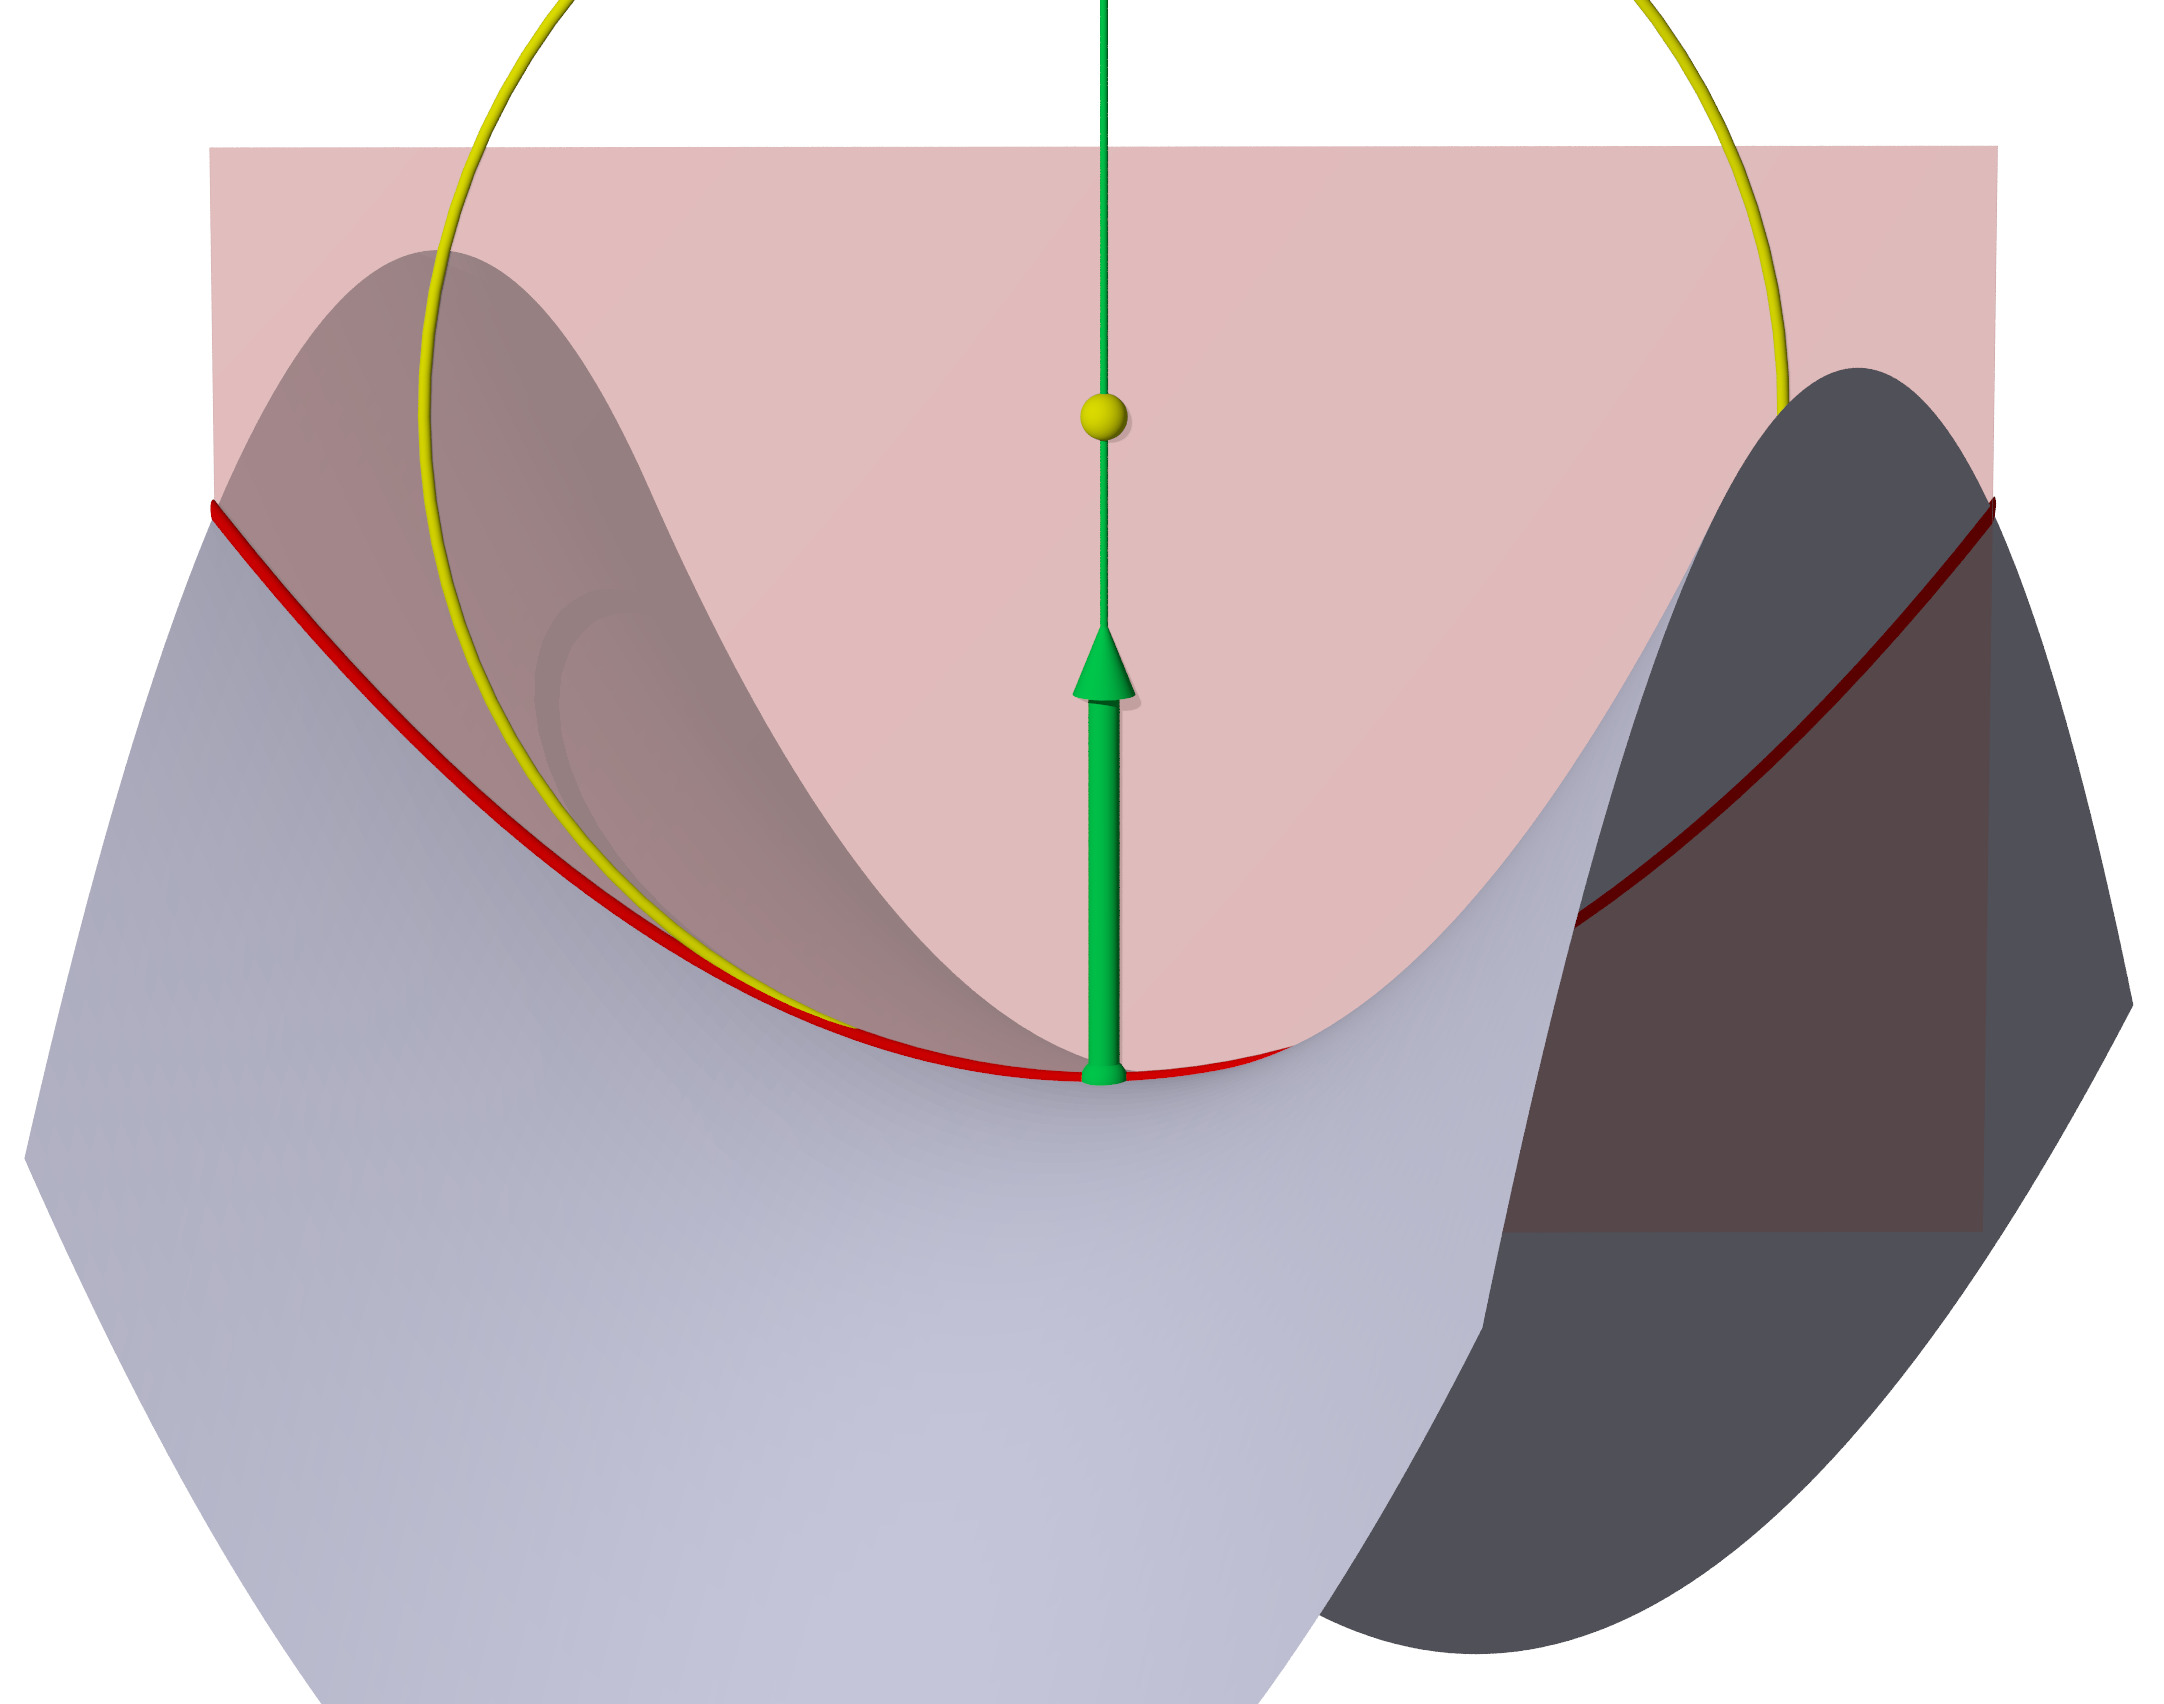
\includegraphics[width=\hsize]{chapters/3d/schnittkruemmung.jpg}
\caption{Die Schnittkrümmung einer Fläche $g(u,v)$ im Punkt $P$ ist
die Krümmung der Schnittkurve (rot) einer Ebene durch $P$, die den
Normalenvektor $n(P)$ (grün) enthält.
Der Krümmungskreis und sein Mittelpunkt $Q$ sind gelb eingezeichnet.
\label{skript:schnittkruemmung}}
\end{figure}
Sei jetzt also eine Fläche $g(u,v)$ gegeben.
Im Punkt $P=g(u_0,v_0)$ betrachten wir Ebenen, die die Normale $n(P)$
enthalten.
Die Schnittkurve der Fläche mit einer solchen Ebene ist eine ebene
Kurve, wir können also deren Krümmung bestimmen
(Abbildung~\ref{skript:schnittkruemmung}).
Es gibt einen Punkt $Q = P + \varrho \cdot n(P)$ in der Ebene, so dass
ein Kreis um den Punkt $Q$ in der Ebene die Krümmung der Kurve bestmöglich
wiedergibt.
Im Gegensatz zur Berechnung der Krümmung in
Abschnitt~\ref{section:kurve:kruemmung}, die immer eine Zahl $\ge 0$
als Wert der Krümmung geliefert hat, spielt es hier das Vorzeichen von
$\varrho$ eine Rolle.
Ist die Kurve in Richtung von $n(P)$ gekrümmt, ist der Punkte $Q$ auf der
gleichen Seite der Fläche wie $n(P)$ und damit $\varrho\ge 0$.
Ist dagegen die Kurve in die Gegenrichtung von $n(P)$ gekrümmt, liegt der
Punkt $Q$ auf der anderen Seite und damit ist $\varrho\le 0$.
Der Punkt $Q$ und der Krümmungskreis sind in
Abbildung~\ref{skript:schnittkruemmung} gelb eingezeichnet.

\begin{beispiel}
\label{skript:sattelbeispiel}
Als Beispiel berechnen wir die Krümmung der Schnittkurve des Graphen
der Funktion
$f(x,y) = x^2-y^2$ im Nullpunkt.
Die Normale $n(0)$ ist der Einheitsvektor in $z$-Richtung, die Schnitt\-ebene
enthält also die $z$-Achse.
Die zulässigen $x$- und $y$-Werte auf der Schnittgeraden sind daher Vielfache
eines Einheitsvektors in der $x$-$y$-Ebene, zum Beispiel $x=t\cos\alpha$
und $y=t\sin\alpha$.
Der Wert von $z$ ist dann
\[
z(t)
=
f(x,y)
=
f(t\cos\alpha,t\sin\alpha)
=
t^2\cos^2\alpha - t^2\sin^2\alpha
=
t^2(\cos^2\alpha - \sin^2\alpha)
=
t^2\cos 2\alpha.
\]
In der Schnittebene ist $t$ massstabsgetreu der Parameter entlang der
horizontalen Achse, $z$ hängt davon quadratisch ab.
Die Krümmung im Nullpunkt kann daher mit der
Formel~\eqref{skript:kruemmung:parabel:scheitel}
berechnet werden,
wir finden
\begin{equation}
\kappa = 2\cos2\alpha
\qquad\Rightarrow\qquad
\varrho = \frac1{2\cos2\alpha}.
\label{skript:kruemmung:sattel}
\qedhere
\end{equation}
\end{beispiel}

Selbstverständlich ist es mit entsprechendem Aufwand möglich, allgemeine
Formeln für die Krümmung der Schnittkurven herzuleiten.
Da wir solche aber nicht explizit brauchen, sondern nur einige wenige
spezielle Eigenschaften, vor allem die Richtungsabhängigkeit, verzichten
wir darauf, diesen Formelapparat zu entwickeln.

\subsection{Richtungsabhängigkeit%
\label{skript:kruemmung:richtungsabhaengigkeit}}
Im Beispiel auf Seite~\pageref{skript:sattelbeispiel} wurde gezeigt, wie
die Krümmung der Schnittkurve von der Richtung der Schnittebene
abhängt.
Dabei entstand die einfache Formel~\eqref{skript:kruemmung:sattel}.
In diesem Abschnitt möchten wir zeigen, dass eine ähnlich einfache
Formel für jede beliebige Fläche gilt.

Gegeben ist also eine Fläche mit Parametrisierung $g(u,v)$, wir möchten
die Krümmungen im Punkte $P=g(u_0,v_0)$ genauer untersuchen.
Offenbar spielt dafür die Lage der Fläche im Raum keine Rolle, wir können
also in einem ersten Schritt das Koordinatensystem so drehen, dass der
Punkt $P$ in den Nullpunkt zu liegen kommt, und dass die $x$-$y$-Ebene des
Koordinatensystems tangential an die Fläche wird.
In dieser Lage lässt sich die Fläche immer als Graph einer Funktion
$z=f(x,y)$ schreiben\footnote{%
Der exakte Beweis dieser intuitiv einleuchtenden Aussage kann mit
dem Satz über implizite Funktionen erfolgen, wir wollen auf die Details
verzichten.}.
Damit haben wir das Problem auf die viel einfachere Situation eines
Graphen reduziert.

Die Funktion $f(x,y)$ kann man als Taylorreihe schreiben, wovon wir nur
die ersten drei Terme hinschreiben wollen
\begin{align*}
f(x,y)
&=
\frac{\partial^2 f}{\partial x^2}x^2
+
2\frac{\partial^2 f}{\partial x\partial y}xy
+
\frac{\partial^2 f}{\partial y^2}y^2
+
o(x^2+y^2)
\\
&=
ax^2 + 2bxy + cy^2 + o(x^2+y^2).
\end{align*}
Die Normale auf die Fläche ist die $z$-Achse, die Schnittebene kann
daher wie im Beispiel wieder durch
\[
x=t\cos\alpha,\quad y=t\sin\alpha
\]
beschrieben werden.
Die Schnittkurve in der Schnittebene hat die Gleichung
\begin{equation}
z
=
(a\cos^2\alpha + 2b\cos\alpha\sin\alpha  + c\sin^2\alpha)t^2
+
\text{Terme dritter Ordnung in $t$}.
\label{skript:kruemmung:klammer}
\end{equation}
Bei der Berechnung der Krümmung braucht man nur die ersten und zweiten
Ableitungen. 
Die erste Ableitung ist ohnehin $0$, die zweiten wird durch die Klammer
im Ausdruck \eqref{skript:kruemmung:klammer} gegeben.
Die Terme dritter Ordnung bleiben nach zweimaligem Ableiten Terme erster
Ordnung, für den Wert $t=0$ fallen sie also weg.
Es bleibt also der quadratische Term als krümmungsbestimmend, wir
können die Formel~\eqref{skript:kruemmung:parabel:scheitel} verwenden, um die
Krümmung in Abhängigkeit von $\alpha$ zu ermitteln.
Wir erhalten
\[
\kappa(\alpha)
=
2(a\cos^2\alpha + 2b\cos\alpha\sin\alpha + c\sin^2 \alpha)
=
2\biggl(
\frac{\partial^2 f}{\partial x^2}\cos^2\alpha
+
2\frac{\partial^2 f}{\partial x\partial y}\cos\alpha\sin\alpha
+
\frac{\partial^2 f}{\partial y^2}\sin^2 \alpha
\biggr).
\]
Die Krümmung einer Schnittkurve in Richtung des Tangentialvektors
$(\cos\alpha,\sin\alpha)$ ist daher durch die zweiten Ableitungen von
$f$ im Punkt $P$ vollständig bestimmt.

\begin{definition}
In jedem Punkt gibt es also eine Abbildung, die jedem
Tangentialeinheitsvektor $e$
die Krümmung der Schnittkurve $\kappa(e)$ einer Ebene durch den Normalenvektor
$n(P)$ und die Tangentenrichrtung $e$ mit der Fläche zuordnet.
Sie heisst die Schnittkrümmung der Fläche in Richtung $e$.
Das Vorzeichen von $\kappa(e)$ ist so gewählt, dass $P+n(P)/\kappa(e)$ der
Mittelpunkt des Krümmungskreises ist.
\end{definition}

%
% hauptkruemmungen.tex
%
% (c) 2017 Prof Dr Andreas Müller, Hochschule Rapperswil
%
\section{Hauptkrümmungen%
\label{skript:kurven:section:hauptkruemmungen}}
In Abschnitt~\ref{skript:kruemmung:richtungsabhaengigkeit} wurde gezeigt,
dass die Schnittkrümmungen $\kappa(e)$ in Abhängigkeit von der
Tangentenrichtung $e$ dank der Wahl eines speziellen Koordinatensystems
mit Hilfe der Matrix der zweiten Ableitung berechnet werden kann.
Wenn $e$ ein Einheitsvektor ist, dann haben wir gefunden, dass die
Schnittkrümmung
\begin{equation}
\kappa(e)
=
2\biggl(
\frac{\partial^2 f}{\partial x^2}
e_1^2
+
2
\frac{\partial^2 f}{\partial x\partial y}e_1e_2
+
\frac{\partial^2 f}{\partial y^2}e_2^2
\biggr)
\label{skript:kurven:ksausdruck}
\end{equation}
ist.
In dieser Form ist nicht klar erkennbar, wie $\kappa(e)$ von $e$ abhängt.
\rhead{Hauptkrümmungen}

Wir können den Ausdruck~\eqref{skript:kurven:ksausdruck} für
$\kappa(e)$ aber auch in Vektorform schreiben.
Dazu schreiben wir die Matrix der zweiten Ableitungen als
\[
H
=
{\def\arraystretch{1.9}
\begin{pmatrix}
\displaystyle\frac{\partial^2 f}{\partial x^2}&
\displaystyle\frac{\partial^2 f}{\partial x\partial y}\\
\displaystyle\frac{\partial^2 f}{\partial x\partial y}&
\displaystyle\frac{\partial^2 f}{\partial y^2}
\end{pmatrix}},
\]
sie heisst die {\em Hessische Matrix}.
\index{Hessische Matrix}%
\index{Matrix, Hessische}%
Damit kann die Krümmung als Matrizenprodukt geschrieben werden:
\[
\kappa(e)
=
\begin{pmatrix}e_1&e_2\end{pmatrix}
{\def\arraystretch{1.9}
\begin{pmatrix}
\displaystyle\frac{\partial^2 f}{\partial x^2}&
\displaystyle\frac{\partial^2 f}{\partial x\partial y}\\
\displaystyle\frac{\partial^2 f}{\partial x\partial y}&
\displaystyle\frac{\partial^2 f}{\partial y^2}
\end{pmatrix}}
\begin{pmatrix}e_1\\e_2\end{pmatrix}
=
e^tHe.
\]
Die Matrix $H$ ist offenbar symmetrisch.

\begin{figure}
\centering
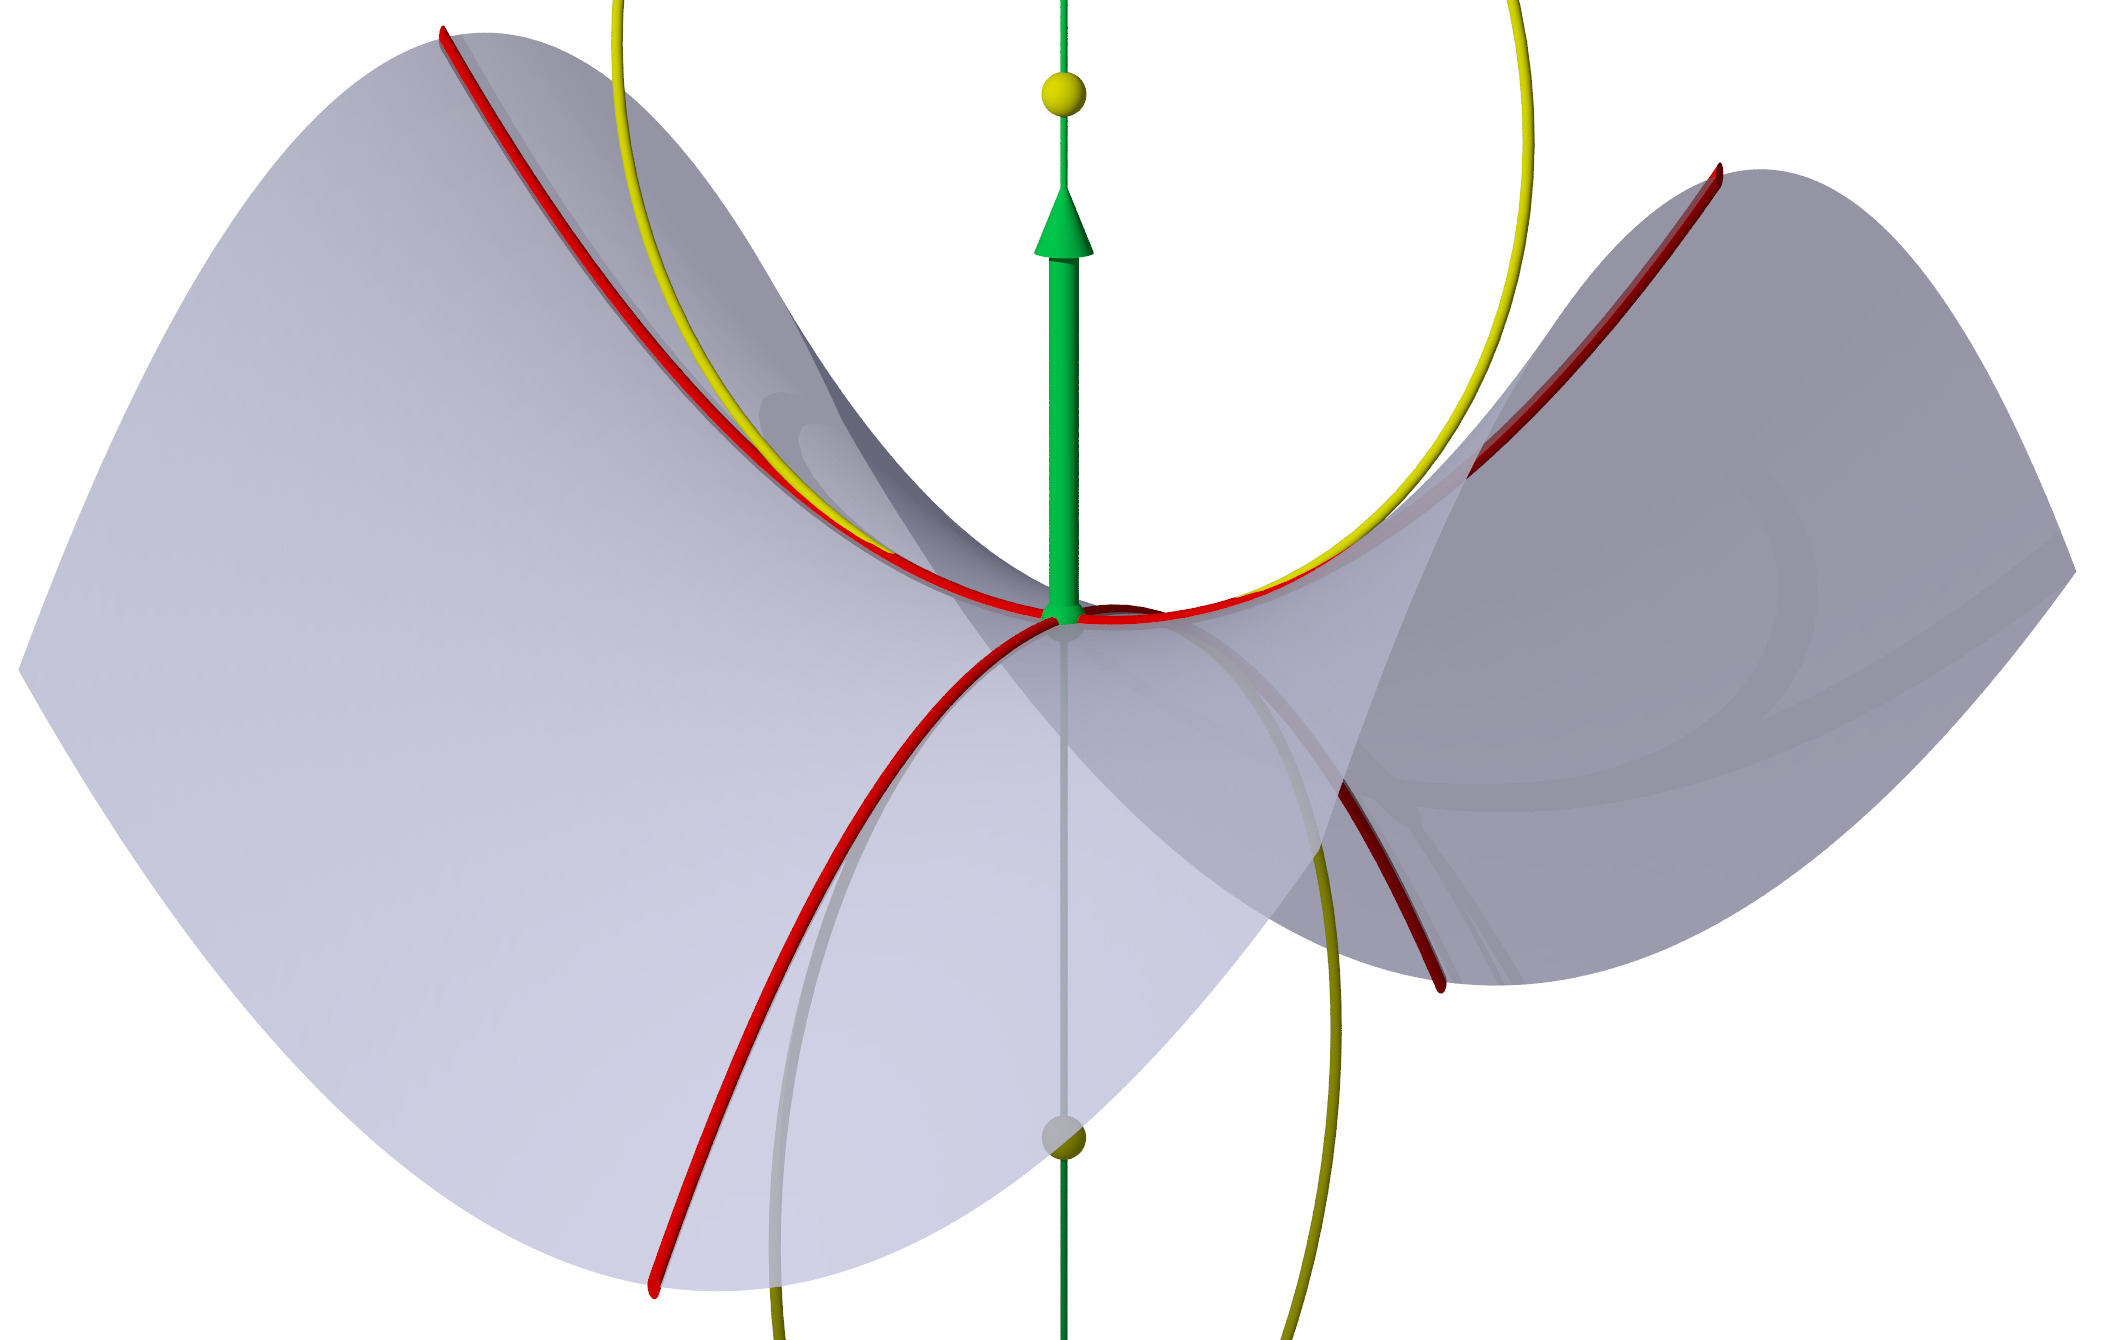
\includegraphics[width=\hsize]{chapters/3d/hauptkruemmungen.jpg}
\caption{Die Hauptkrümmungen einer Fläche sind die maximale und minimale
Schnittkrümmung in einem Punkte.
Die zugehörigen Krümmungsrichtungen heissen die Hauptkrümmungsrichtungen.
In diesem Beispiel haben die beiden Hauptkrümmungen verschiedenes Vorzeichen.
\label{skript:kurven:hauptkruemmungen}}
\end{figure}

In der linearen Algebra lernt man, dass sich jede symmetrische Matrix 
mit Hilfe einer Matrix in $\textrm{SO}(n)$ diagonalisieren lässt.
Auf den vorliegenden Fall angewendet gibt es eine Drehung der
$x$-$y$-Ebene derart, dass
die Matrix $H$ Diagonalform bekommt.
Wir wählen das Koordinatensystem daher so, dass die
Krümmung in Abhängigkeit vom Einheitsvektor $e$ durch
\[
\kappa(e)
=
2\lambda_1 e_1^2 + 2\lambda_2 e_2^2
\]
beschrieben wird,
wobei $\lambda_1$ und $\lambda_2$ die Eigenwerte von $H$ sind.
Für $e_1=\cos\alpha$ und $e_2=\sin\alpha$ bekommt man
\[
\kappa(\alpha)
=
2\lambda_1 \cos^2\alpha + 2\lambda_2 \sin^2\alpha.
\]
Diese Funktion nimmt ihr Maximum und Minimum auf den Achsen an,
die Eigenwerte sind also bis auf den Faktor $2$ die maximale und minimale
Schnittkrümmung.
Wir schreiben $\kappa_1=2\lambda_1$ und $\kappa_2=2\lambda_2$ für die
beiden zugehörigen Krümmungen.
\index{Hauptkrümmungen}%
Diese heissen auch die Hauptkrümmungen, die Richtungen der Achsen heissen
die Hauptkrümmungsrichtung, und sie stehen senkrecht aufeinander, weil
\index{Hauptkrümmungsrichtung}%
die Eigenvektoren einer symmetrischen Matrix zu verschiedenen Eigenvektoren
immer senkrecht aufeinander stehen.

\subsection{Invarianten}
Die hessische Matrix $H$ hat die Eigenwerte $\lambda_1$ und $\lambda_2$.
Als einzelne Werte sind diese nicht so interessant.
Hingegen sind die Determinante und die Spur von $H$ Invarianten, die
unabhängig von der Wahl des Koordinatensystems sind.

\subsubsection{Determinante --- Gausskrümmung}
\index{Gausskrümmung}%
\index{Krümmung!Gauss-}%
\index{Determinante}%
Die Determinante von $H$ ist das Produkt der Eigenwerte, also
\[
\det H
=
\lambda_1\lambda_2
=
\frac14 (2\lambda_1) (2\lambda_2)
=
\frac14 \kappa_1\kappa_2.
\]
\begin{definition}
\label{skript:definition:gausskruemmung}
Das Produkt der Hauptkrümmungen $K=\kappa_1\kappa_2$
heisst {\em Gausskrümmung} der Fläche.
\end{definition}
Es stellt sich heraus, dass die Gausskrümmung auch aus inneren Eigenschaften
der Fläche ermittelt werden kann
(Theorema Egregium von Gauss).
Wir werden in Kapitel~\ref{skript:chapter:kruemmung} 
mit der Riemannschen Krümmung ein Konzept der Krümmung eines Raumes
definieren, welches für Flächen im Wesentlichen mit der Gausskrümmung
übereinstimmt.

\subsubsection{Spur --- mittlere Krümmung}
\index{mittlere Krümmung}%
\index{Krümmung!mittlere}%
\index{Spur}%
Die Spur von $H$ ist eine weitere Invariante der Hessischen Matrix.
Es gilt
\[
\operatorname{Spur} H
=
\lambda_1+\lambda_2
=
\frac12(2\lambda_1+2\lambda_2)
=
\frac12(\kappa_1+\kappa_2).
\]
In Abschnitt~\ref{skript:kurve:mittlerekruemmung} haben wir nachgeweisen,
dass die mittlere Krümmung gleichzeitig die Spur der Hessischen Matrix ist.
Obige Überlegung zeigt, dass dies auch der Mittelwert der Hauptkrümmungen ist.
Dies führt auf die folgende alternative Definition der mittleren Krümmung.

\begin{definition}
\label{skript:definition:mittlerekruemmung2}
Die {\em mittlere Krümmung} ist auch der Mittelwert
\[
M=\frac12(\kappa_1+\kappa_2)
\]
der Hauptkrümmungen.
\end{definition}
Die mittlere Krümmung ist wichtig zur Charakterisierung von Minimalflächen
im Kapitel~\ref{chapter:minimal}.

\subsection{Gausskrümmung und Flächeninhalt%
\label{skript:kurven:gaussflaeche}}
Die mittlere Krümmung $M$ hat eine einfach geometrische Interpretation
als Mittelwert aller Schnittkrümmungen.
Sie zeigt auch ganz offensichtlich, dass sie eine Eigenschaft der Einbettung
einer Fläche in den dreidimensionalen Raum ist.
Für die Gausskrümmung fehlt uns eine vergleichbare Charakterisierung.
Wir wollen daher in diesem Abschnitt zeigen, dass die Gausskrümmung
mit der Längenmessung entlang eines kleinen Kreises um den Nullpunkt
zusammenhängt.
Da sowohl die Länge wie auch der Flächeninhalt unabhängig von der
Einbettung gemessen werden kann,
wird dies auch gleichzeitig illustrieren, dass die Gausskrümmung eine
innere Eigenschaft einer Fläche ist.

\begin{figure}
\centering
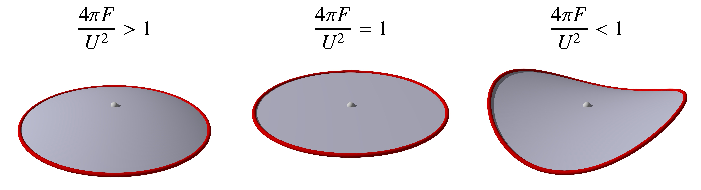
\includegraphics{chapters/tikz/4pifu2.pdf}
\caption{Das Verhältnis von Flächeninhalt zu Umfang im Quadrat einer
kleinen Kreisscheibe hängt von der Gausskrümmung ab. 
Für eine Flache Kreisscheibe gilt $4\pi F/U^2=1$ (Mitte).
Bei positiver Gausskrümmung (links) ist der Umfang gleich, der Flächeninhalt
aber grösser, daher wird das Verhältnis grösser.
Bei negativer Gausskrümmung (rechts) wird der Umfang deutlich länger, so dass
das Verhältnis kleiner wird.
\label{skript:kurven:4pifu2vis}}
\end{figure}
Dazu betrachten wir wieder eine Fläche der Form $z=f(x,y)$, deren
Tangentialebene im Nullpunkt die $x$-$y$-Ebene ist.
In dieser Fläche betrachten wir den Kreis parametrisiert mit
$x=R\cos t$ und $y=R\sin t$.
In einer Ebene wird der Flächeninhalt $F=\pi R^2$ sein, der Umfang $U=2\pi R$.
Man kann auch sagen, dass
\[
U^2 = 4\pi F
\qquad\Rightarrow\qquad
\frac{4\pi F}{U^2}=1
\]
ist.
Wir untersuchen, wie sich diese Beziehung ändert, wenn die
Fläche nicht mehr eine Ebene ist (Abbildung~\ref{skript:kurven:4pifu2vis}).

Wir approximieren die Fläche wieder als quadratische Funktion.
Zur Vereinfachung der Rechnung verwenden wir dabei ein Koordinatensystem,
in dem die Hauptrkümmungsrichtungen die Achsen sind.
Die Funktion $f(x,y)$ hat daher die Form
\[
f(x,y)
=
\kappa_1 x^2 + \kappa_2 y^2
\qquad\text{und}\qquad
g(x,y)=\begin{pmatrix}x\\y\\\kappa_1x^2 + \kappa_2y^2\end{pmatrix}.
\]
Für diese Fläche berechnen wir jetzt Flächeninhalt $F$ und 
Umfang $U$.

\subsubsection{Flächeninhalt}
Der Flächeninhalt einer mit $(u,v)$ parametrisierten Fläche $g(u,v)$
wird mit dem Integral
\[
F
=
\int_{D}
\biggr|\frac{\partial g}{\partial u} \times \frac{\partial g}{\partial v}\biggr|
\,du\,dv
\]
über das Definitionsgebiet $D$ der Fläche berechnet.
In unserem Fall verwenden wir $x$ und $y$ als Parameter und das
Definitionsgebiet
\[
D_R = \{ (x,y)\;|\; x^2 + y^2 < R\}.
\]
Der Betrag des Vektorprodukts im Integranden ist in unserem Fall
\begin{align*}
\biggl|
\frac{\partial g}{\partial x}
\times
\frac{\partial g}{\partial y}
\biggr|
&=
\left|
\begin{pmatrix}1\\0\\\frac{\partial f}{\partial x}\end{pmatrix}
\times
\begin{pmatrix}0\\1\\\frac{\partial f}{\partial y}\end{pmatrix}
\right|
=
\left|
\begin{pmatrix}1\\0\\2\kappa_1 x\end{pmatrix}
\times
\begin{pmatrix}0\\1\\2\kappa_2 y\end{pmatrix}
\right|
=
\left|
\begin{pmatrix}-2\kappa_1 x\\-2\kappa_2 y\\1
\end{pmatrix}
\right|
\\
&=
1 + 4\kappa_1^2 x^2 + 4 \kappa_2^2 y^2.
\end{align*}
Da das Integrationsgebiet eine Kreisscheibe mit Radius $R$ ist, verwenden
wir mit Vorteil Polarkoordinaten.
Wir ersetzen $x=r\cos\varphi$, $y=r\sin\varphi$ und $dx\,dy = r\,dr\,d\varphi$
und schreiben das Integral als
\begin{align*}
F
&=
\int_0^{2\pi}
\int_0^R
\sqrt{1 + 4\kappa_1^2 r^2 \cos^2 \varphi + 4\kappa_2^2 r^2\sin^2\varphi}
\,
r\,dr\,d\varphi
\end{align*}
Der Integrand ist leider zu kompliziert, um das Integral in geschlossener
Form derart auszuwerten, dass wir daraus die beabsichtigten Schlüsse
ziehen können.
Da wir aber schon bei der Funktion $f(x,y)$ nur mit einer Approximation
für kleine Werte von $r$ arbeiten, können wir den Integranden in eine
Taylorreihe in $r$ entwickeln.
Die Rechnung mit dem Maxima Programm
\lstinputlisting[style=Maxima]{chapters/listings/flaecheninhalt.maxima}
ergibt
\begin{align*}
F
%&=
%\int_0^{2\pi}
%\int_0^R
%\frac12R^2(1+R^2\kappa_1^2 \cos^2\varphi + R^2 \kappa_2^2\sin^2\varphi)
%\,r\,dr\,d\varphi
%\\
&=
\pi R^2
\bigl(
1
+
{\textstyle\frac12} R^2(\kappa_1^2+\kappa_2^2)
\bigr).
\end{align*}
Der erste Terme ist natürlich exakt der Flächeninhalt einer Kreisscheibe
in der Ebene.

\subsubsection{Umfang}
Für den Umfang berechnen wir das Wegintegral entlang des Randes.
Um eine Parametrisierung der Randkurve zu bekommen,
ersetzen wir $x=R\cos t$ und $y=R\sin t$ in $g(x,y)$ und erhalten
\[
c(t)
=
\begin{pmatrix}
R\cos t\\ R\sin t\\ R^2(\kappa_1^2\cos^2 t + \kappa_2^2\sin^2 t)
\end{pmatrix}
=
R
\begin{pmatrix}
\cos t\\ \sin t\\ R(\kappa_1^2\cos^2 t + \kappa_2^2\sin^2 t)
\end{pmatrix}.
\]
Wir müssen den Betrag der Ableitung $\dot c(t)$ integrieren.
Das ist das Integral
\begin{align*}
U
&=
R
\int_0^{2\pi}
\sqrt{
\sin^2 t + \cos^2 t 
+ R^2(\kappa_1^2 \cos^2 t + \kappa_2^2\sin^2 t)
}
\,dt,
\end{align*}
welches sich ebenfalls nicht in geschlossener Form auswerten lässt.
Auch hier wählen wir wieder die Entwicklung in eine Taylorreihe nach $R$,
denn wir brauchen $U$ ja nur für kleine Werte von $R$.
Die Rechnung mit dem Maxima Programm
\lstinputlisting[style=Maxima]{chapters/listings/umfang.maxima}
gibt wieder
\begin{align}
U
&\simeq
R
\int_0^{2\pi}
1 + 2(\kappa_1^2 - 2\kappa_1\kappa_2 + \kappa_2^2)R^2 \cos^2 t\sin^2 t
\,dt
\notag
\\
&=
2\pi R
(
1
+ 
{\textstyle \frac14}(\kappa_1^2 -2\kappa_1\kappa_2+\kappa_2^2) R^2
).
\label{skript:kurven:U1}
\end{align}
Für die Beziehung zwischen Umfang und Flächeninhalt brauchen wir aber nicht
$U$ sondern sein Quadrat (auch dies wird im oben gelisteten Programm bereits
berechnet).
In unserer Näherung brauchen wir dabei nur Terme bis zur vierten Ordnung
in $R$ zu berücksichtigen.
Wegen $(1+x)^2 \simeq 1+2x$ in niedrigster Ordnung, bedeutet das nur,
dass wir den zweiten Term in der Klammer in \eqref{skript:kurven:U1}
verdoppeln müssen.
Wir bekommen daher
\begin{align*}
U^2
&\simeq
4\pi^2 R^2(
1
+
{\textstyle \frac12}
(\kappa_1^2-2\kappa_1\kappa_2 + \kappa_2^2)R^2
)
\end{align*}
als Approximation in niedrigster Ordnung.

\subsubsection{Beziehung zwischen Umfang und Flächeninhalt}
Wir müssen die Grösse $4\pi F/U^2$ untersuchen.
Mit den bisher berechneten Ausdrücken für $F$ und $U$ erhalten wir
\begin{align}
\frac{4\pi F}{U^2}
&=
\frac{4\pi^2R^2(1+{\textstyle\frac12}(\kappa_1^2 + \kappa_2^2)R^2)}%
{4\pi^2 R^2(1+{\textstyle\frac12}(\kappa_1^2-2\kappa_1\kappa_2+\kappa_2^2)R^2)}
=
\frac{1+(\kappa_1^2 + \kappa_2^2)R^2}%
{1+(\kappa_1^2-2\kappa_1\kappa_2+\kappa_2^2)R^2}.
\label{skript:kurven:4piu2}
\end{align}
Wieder brauchen wir nur eine Taylorreihe bis zur zweiten Ordnung in $R$.
Mit Hilfe der geometrischen Reihe 
\[
\frac1{1+x}= 1-x+x^2-x^3+\dots
\]
können wir den Nenner in~\eqref{skript:kurven:4piu2} in den Zähler
bringen.
Wenn wir wieder Terme höherer Ordnung als $R^2$ weglassen, bekommen
wir 
\begin{equation}
\frac{4\pi F}{U^2}
\simeq
1+\kappa_1\kappa_2R^2
=
1 + KR^2
\end{equation}
als Schlussresultat.
Das Produkt der Hauptkrümmungen ist die Gausskrümmung $K=\kappa_1\kappa_2$.
Die Gausskrümmung beschreibt also im Wesentlichen das Anwachsen des
Verhältnisses von Flächeninhalt zu Umfang im Quadrat eines Kreises
in Abhängigkeit von dessen Radius.
Bei positiver Gauss\-krümmung wächst das Verhältnis schneller an
als in einer Ebene, bei negativer Gausskrümmung langsamer.







\section*{Übungsaufgaben}
\rhead{Übungsaufgaben}
\uebungsaufgabe{0101}

